\documentclass{standalone}
%% Show/hide steps for standalone work — edit this line:
\makeatletter\AtBeginDocument{\@buildstepset{0,1,2,3,4}}\makeatother
\usepackage{tikz}
\usetikzlibrary{intersections,calc,backgrounds}
\usepackage{amsmath}
\usepackage{hsbcommon}
\begin{document}
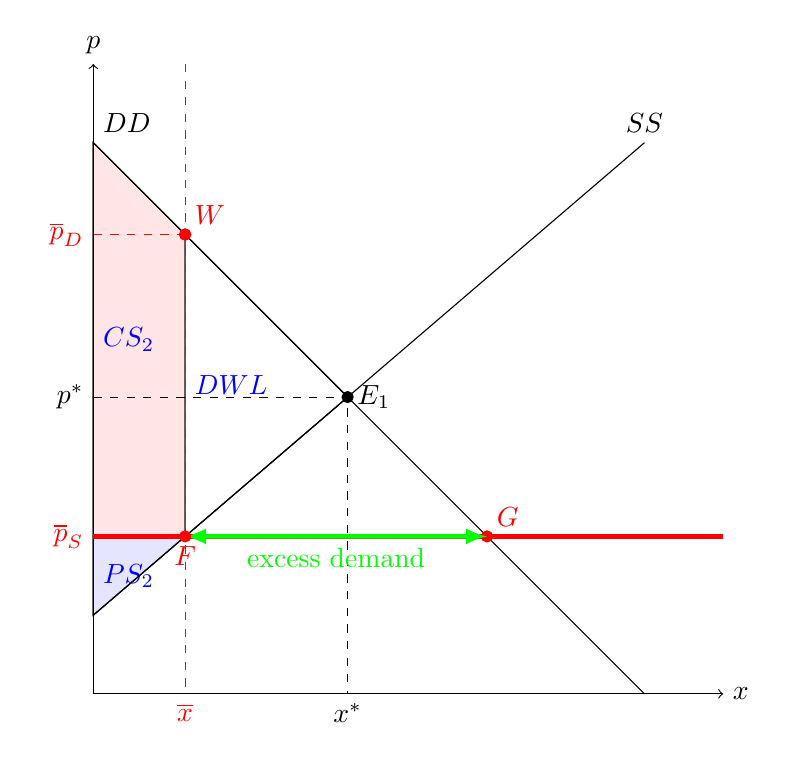
\begin{tikzpicture}
% \tikzset{>=latex,every node/.style={opacity=0}}
    \draw[->] (0,0) node[below] {\phantom{$X_i$}} -- (8,0) node [opacity=1,right] {$x$};
    \draw[->] (0,0) node[left] {\phantom{$Y_mi$}} -- (0,8) node [opacity=1,above] {$p$};

    %% ── All coordinates unconditional ────────────────────────────────────────
    \coordinate (A) at (0,7);
    \coordinate (B) at (7,0);
    \coordinate (E) at (0,1);
    \coordinate (F) at (7,7);
    \coordinate (G) at (0,2);   % price ceiling on p-axis
    \coordinate (H) at (8,2);   % price ceiling right end

    %% ── Named paths ──────────────────────────────────────────────────────────
    \draw[name path global=demand]   plot [smooth] coordinates {(A)(B)};
    \draw[name path global=supply]   plot [smooth] coordinates {(E)(F)};
    \path[name path global=ceiling,red]  plot [smooth] coordinates {(G)(H)};

    %% ── All intersections pre-computed ───────────────────────────────────────
    \path [name intersections={of=demand and supply,  by=X}];  % free-market eq.
    \path [name intersections={of=demand and ceiling, by=Y}];  % demand at ceiling
    \path [name intersections={of=supply and ceiling, by=Z}];  % supply at ceiling

    %% vertical at Z for quantity supplied under ceiling
    \path[name path global=quantity] (Z |-,8) -- (Z |-,0);
    \path [name intersections={of=demand and quantity, by=R}]; % demand at Q_Z

    %% ── Always visible: free-market equilibrium ──────────────────────────────
    \node[opacity=1,above right] at (A) {$DD$};
    \node[opacity=1,above]       at (F) {$SS$};

    \draw[dashed] (0,|- X) node [left] {$p^*$} -- (X) -- (X |-,0) node [below] {$x^*$};

    \filldraw (X) node[right] {$E_1$} circle (2pt);

    %% ── Step 2: original welfare ─────────────────────────────────
    \ifstep{1}{
        \begin{scope}[on background layer]
            \draw[fill=red!10]  (A) -- (X) -- (0,|- X) -- node[right] {$CS_1$} cycle;
            \draw[fill=blue!10] (E) -- (X) -- (0,|- X) -- node[right] {$PS_1$} cycle;            
        \end{scope}
    
    }
 
     %% ── Step 2: price ceiling ─────────────────────────────────
    \ifstep{2}{
            \draw[red,name path global=ceiling, ultra thick] plot [smooth] coordinates {(G)(H)};
    }

    
    %% ── Step 3: price ceiling, excess demand ─────────────────────────────────
    \ifstep{3}{
        \begin{scope}[color=red]
            \node[left] at (G) {$\overline{p}_{S}$};
            \draw[name path global=ceiling, ultra thick] plot [smooth] coordinates {(G)(H)};
            \filldraw (Y) node[above right] {$G$} circle (2pt);
            \draw[dashed, name path global=quantity] (Z |-,8) -- (Z |-,0);
            \filldraw (R) circle (2pt);
            \draw[<->,>=latex,ultra thick,color=green] (Z) -- node[below] {excess demand} (Y);
            \filldraw (Z) node[below] {$F$} circle (2pt);
            \filldraw (R) node[above right] {$W$} circle (2pt);
            \draw[dashed] (R|-,0) node [below] {$\overline{x}$} (R) -- (0,|-R) node[left] {$\overline{p}_{D}$};
        \end{scope}
    }

    %% ── Step 4: welfare areas under ceiling ──────────────────────────────────
    \ifstep{4}{
        \begin{scope}[color=blue, on background layer]
            \draw[fill=red!10]  (A) -- (R) -- (Z) -- (G) -- node[right] {$CS_2$} cycle;
            \draw[fill=blue!10] (G) -- (Z) -- (E) -- node[right] {$PS_2$} cycle;
            \draw[fill=white]   (R) -- (X) -- (Z) -- node[right] {$DWL$}  cycle;
        \end{scope}
    }

\end{tikzpicture}
\end{document}